\documentclass{article}
\usepackage{graphicx}
\usepackage{tikz,float}
\usepackage{amsmath,amsthm}
\usepackage[capitalize]{cleveref}
\usetikzlibrary{positioning}

\newtheorem{case}{Case}
\newtheorem{subcase}{Case}
\numberwithin{subcase}{case}

\title{$\aleph_{0}$ Weekly Problem}
\author{Ravi Dayabhai \& Conrad Warren}
\date{2024-07-31}

\begin{document}
\maketitle

\section*{Problem}

In a group of nine people, one person knows two of the others, two people each know four others, four each know five others, and the remaining two each know six others. Show that there are three people who all know each other.

\section*{Solution}

\begin{proof}

We will proceed by casework, modeling the problem as an undirected graph on nine vertices (corresponding the individuals) wherein any edge represents the ``knows'' relation between the two individuals corresponding to the edge's incident vertices. We will show there exists a clique of size three on this undirected graph\footnote{The ``knows'' relation is assumed to be symmetric because the claim we intend to prove does not always hold for a directed graph.}.

Let vertices $A_{1}$ and $A_{2}$ represent the two individuals who know six others (read: $A$-vertices). The remaining seven vertices (corresponding to the individuals who know fewer than six others) are labeled $B_{1}, B_{2}, \ldots, B_{7}$  (read: $B$-vertices).

\begin{case}[The edge $(A_{1}, A_{2})$ exists.]

    When edge $(A_{1}, A_{2})$ exists, there are a total of $10$ remaining edges that are incident to an $A$-node and a $B$-node. By the Pigeonhole Principle, there exists a vertex $B_{*}$ that must neighbor both $A_{1}$ and $A_{2}$. A clique of size three exists since there are edges connecting all pairs taken from $\lbrace A_{1}, A_{2}, B_{*} \rbrace$. For example, in \cref{fig:case_1}, $B_{*}$ can be $B_{3}$, $B_{4}$, or $B_{5}$.

    \begin{figure}[H]
        \centering
        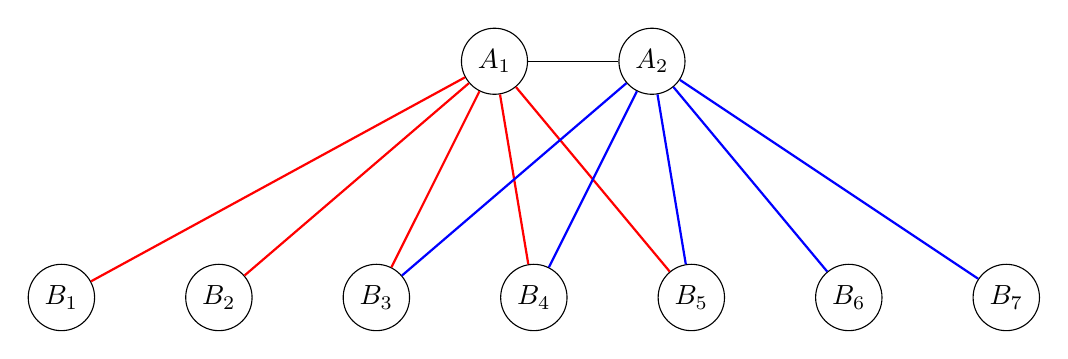
\begin{tikzpicture}
        % Nodes
        \node (n1) at (-1.5,3) [circle, draw] {\(A_1\)};
        \node (n2) at (0.5,3) [circle, draw] {\(A_2\)};
        \node (n3) at (-7,0) [circle, draw] {\(B_1\)};
        \node (n4) at (-5,0) [circle, draw] {\(B_2\)};
        \node (n5) at (-3,0) [circle, draw] {\(B_3\)};
        \node (n6) at (-1,0) [circle, draw] {\(B_4\)};
        \node (n7) at (1,0) [circle, draw] {\(B_5\)};
        \node (n8) at (3,0) [circle, draw] {\(B_6\)};
        \node (n9) at (5,0) [circle, draw] {\(B_7\)};
        % Lower nodes
        
        % Edges
        \foreach \i in {3,4,5,6,7} {
            \draw[red, thick] (n1) -- (n\i);
        }
        \foreach \i in {5,6,7,8,9} {
            \draw[blue, thick] (n2) -- (n\i);
        }
        
        \draw (n1) -- (n2);
    \end{tikzpicture}
    \caption{Edge $(A_{1}, A_{2})$ exists.}
    \label{fig:case_1}
    \end{figure}

\end{case}

\begin{case}[The edge $(A_{1}, A_{2})$ does not exist.]

There are two sub-cases to consider when edge $(A_{1}, A_{2})$ does not exist.

\begin{subcase}[The edge $(A_{1}, A_{2})$ does not exist and $A$-nodes share the same set of neighbors.]

Without loss of generality, let vertex $B_{7}$ be the node not connected to either of the $A$-vertices (see \cref{fig:case_21}). For all  $(u, v) \in \lbrace B_{1}, B_{2}, \ldots, B_{6} \rbrace$, if edge $(u, v)$ exists, a clique of size three exists (namely, among either $A$-vertex, $u$, and $v$). 

By the Pigeonhole Principle, there exists $B_{*} \in \lbrace B_{1}, B_{2}, \ldots, B_{6} \rbrace$ that has degree four, as the problem states two nodes have degree four. Since there exists two edges that are both incident to $B_{*}$ and neither of which is incident to an $A$-node, at least one of these edges must connect to a vertex in $\lbrace B_{1}, B_{2}, \ldots, B_{6} \rbrace \setminus \lbrace B_{*} \rbrace$ (again, by the Pigeonhole Principle). This results in some edge $(u, v) \in \lbrace B_{1}, B_{2}, \ldots, B_{6} \rbrace \setminus \lbrace B_{*} \rbrace \subset \lbrace B_{1}, B_{2}, \ldots, B_{6} \rbrace$ existing and, therefore, a clique of size three existing.

    \begin{figure}[H]
        \centering
        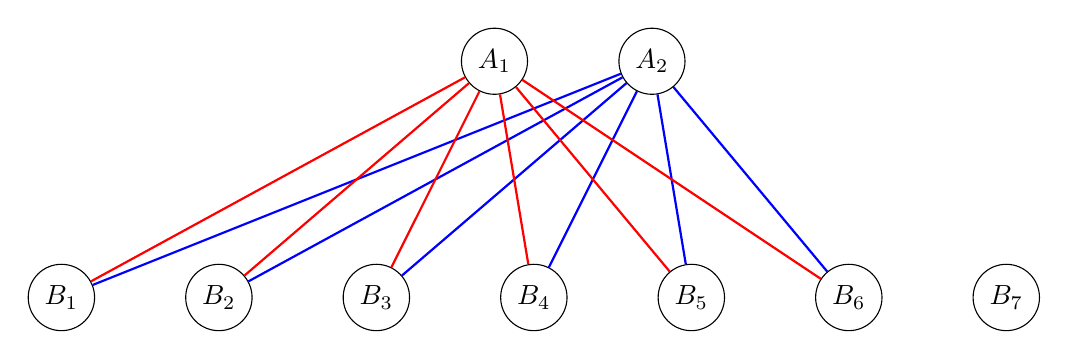
\begin{tikzpicture}
        % Nodes
        \node (n1) at (-1.5,3) [circle, draw] {\(A_1\)};
        \node (n2) at (0.5,3) [circle, draw] {\(A_2\)};
        \node (n3) at (-7,0) [circle, draw] {\(B_1\)};
        \node (n4) at (-5,0) [circle, draw] {\(B_2\)};
        \node (n5) at (-3,0) [circle, draw] {\(B_3\)};
        \node (n6) at (-1,0) [circle, draw] {\(B_4\)};
        \node (n7) at (1,0) [circle, draw] {\(B_5\)};
        \node (n8) at (3,0) [circle, draw] {\(B_6\)};
        \node (n9) at (5,0) [circle, draw] {\(B_7\)};
        % Lower nodes
        
        % Edges
        \foreach \i in {3,4,5,6,7,8} {
            \draw[red, thick] (n1) -- (n\i);
            \draw[blue, thick] (n2) -- (n\i);
        }
        
    \end{tikzpicture}
    \caption{The edge $(A_{1}, A_{2})$ does not exist and $A$-nodes share the same set of neighbors.}
    \label{fig:case_21}
    \end{figure}

\end{subcase}

\begin{subcase}[The edge $(A_{1}, A_{2})$ does not exist and $A$-nodes do not share the same set of neighbors.]

Without loss of generality, let node $A_{1}$ connect to six $B$-vertices $\lbrace B_{1}, B_{2}, \ldots, B_{6}\rbrace$. Since $A_{2}$ cannot connect to the same set of $B$-vertices, $B_{7}$ must neighbor $A_{2}$, as do  five vertices in the set of $B$-vertices adjacent to $A_{1}$ due to the Pigeonhole Principle; without loss of generality, let this subset of the neighbors of vertex $A_{1}$ be $\lbrace B_{2}, B_{3}, \ldots, B_{6}\rbrace$ (see \cref{fig:case_22}).

Since two $B$-vertices must have degree four, at least one must be in $\lbrace B_{1}, B_{2}, \ldots, B_{6} \rbrace$ by the Pigeonhole Principle. But having one vertex $B_{*} \in \lbrace B_{1}, B_{2}, \ldots, B_{6} \rbrace$ with degree four necessarily means there exists an edge between $B_{*}$ and a vertex $B_{**} \in \lbrace B_{1}, B_{2}, \ldots, B_{6} \rbrace \setminus \lbrace B_{*} \rbrace$ by the Pigeonhole Principle. This edge creates a clique of size three, consisting of the vertices $B_{*}$, $B_{**}$, and a common neighbor found in $\lbrace A_{1}, A_{2} \rbrace$.


    \begin{figure}[H]
        \centering
        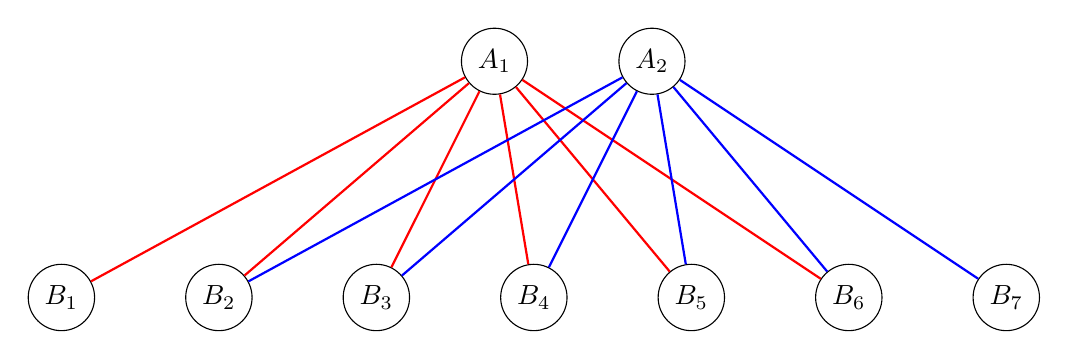
\begin{tikzpicture}
        % Nodes
        \node (n1) at (-1.5,3) [circle, draw] {\(A_1\)};
        \node (n2) at (0.5,3) [circle, draw] {\(A_2\)};
        \node (n3) at (-7,0) [circle, draw] {\(B_1\)};
        \node (n4) at (-5,0) [circle, draw] {\(B_2\)};
        \node (n5) at (-3,0) [circle, draw] {\(B_3\)};
        \node (n6) at (-1,0) [circle, draw] {\(B_4\)};
        \node (n7) at (1,0) [circle, draw] {\(B_5\)};
        \node (n8) at (3,0) [circle, draw] {\(B_6\)};
        \node (n9) at (5,0) [circle, draw] {\(B_7\)};
        % Lower nodes
        
        % Edges
        \foreach \i in {3,4,5,6,7,8} {
            \draw[red, thick] (n1) -- (n\i);
        }
        \foreach \i in {4,5,6,7,8,9} {
            \draw[blue, thick] (n2) -- (n\i);
        }
        
    \end{tikzpicture}
    \caption{The edge $(A_{1}, A_{2})$ does not exist and $A$-nodes do not share the same set of neighbors.}
    \label{fig:case_22}
    \end{figure}
    
\end{subcase}

\end{case}

We have shown via casework that there always exists a group of three individuals that all know each other by demonstrating that a clique of size three exists in the undirected graph modeling the set of relationships described in the problem statement.

\end{proof}
\end{document}
